\chapter{Grundlagen}


\section{Unterteilungsalgorithmen Übersicht}

Unterteilungsalgorithmen erzeugen aus einem Ausgangspolygonnetz eine glatte Fläche.
Die glatte Zielfläche ist dabei der Grenzwert eines unendlichen, rekursiven Verfeinerungsschemas.
\autoref{fig:sd} visualisiert die Anwendung eines Unterteilungsalgorithmus auf eine Kurve und auf eine Fläche.
Nach mehrfacher Anwendung der Unterteilung konvergiert die Kurve oder Fläche gegen die glatte Zielkurve bzw. Zielfläche.

\begin{figure}
  \centering
  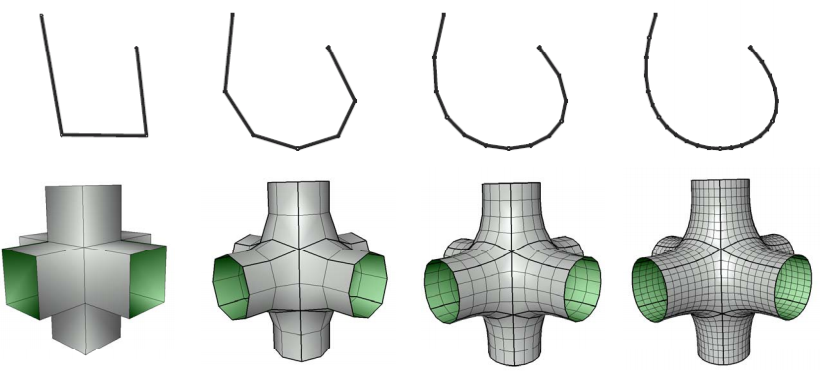
\includegraphics[width=0.8\textwidth]{content/media/sd.png}
  \caption{Unterteilungsalgorithmus - Kurve und Fläche \cite{Standford.24.07.2015}}
  \label{fig:sd}
\end{figure}

Unterteilungsalgorithmen kann man anhand ihrer Eigenschaften Kategorisieren.
Ein Unterscheidungskriterium betrifft die Art und Weiße, wie unterteilt wird.
Man unterscheidet dabei zwischen \emph{Primal} und \emph{Dual}.

\begin{description}
 \item[Primal] Bei dieser Strategie wird die Oberfläche unterteilt (\enquote{face split}).
\autoref{fig:sd_primal} stellt diese Methode für ein Dreicksnetz und ein Vierecksnetz dar.
 \item[Dual] Auf der anderen Seite ist es möglich Eckpunkte in mehrere Eckpunkte aufzusplitten (\enquote{vertex split}).
 Diese Methode ist in \autoref{fig:sd_dual} abgebildet.

\end{description}
\begin{figure}
  \centering
  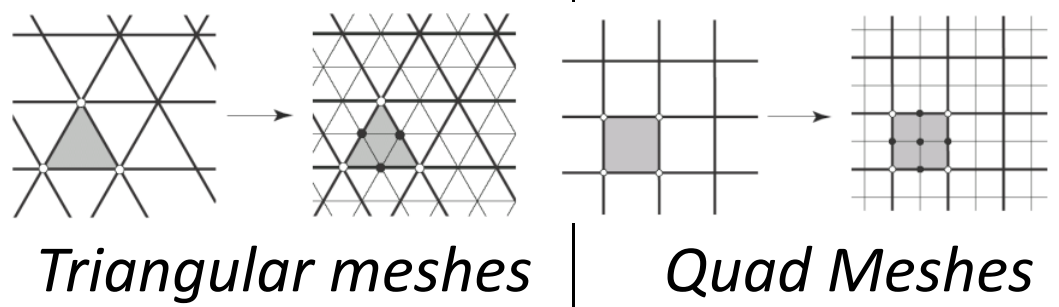
\includegraphics[width=0.7\textwidth]{content/media/sd_primal}
  \caption{Primal (face split) \cite{Standford.24.07.2015}}
  \label{fig:sd_primal}
\end{figure}

\begin{figure}
  \centering
  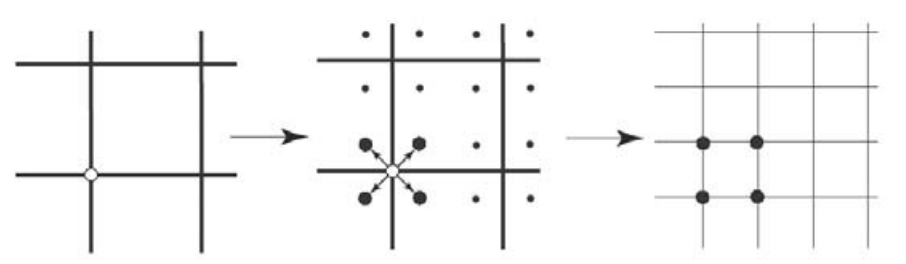
\includegraphics[width=0.7\textwidth]{content/media/sd_dual}
  \caption{Dual (vertex split) \cite{Standford.24.07.2015}}
  \label{fig:sd_dual}
\end{figure}

Ein weiteres wesentliches Merkmal ist, ob Kontrollpunkte interpoliert werden oder nicht. 
\begin{description}
 \item[Approximation] Kontrollpunkte werden nicht interpoliert.
 \item[Interpolation] Kontrollpunkte werden interpoliert.
\end{description}

\autoref{tab:sd_comp} listet die bekanntesten Unterteilungsalgorithmen auf und ordnet diese den Kategorien zu.
Zu jedem Algorithmus ist zusätzlich die \enquote{Glattheit} der Oberfläche angegeben (C-Stetigkeit).
Dies kann auch als Maß über die Qualität des Unterteilungsalgorithmus fungieren.


\begin{table}
\center
\caption{Unterteilungsalgorithmen Übersicht}
\label{tab:sd_comp}
\begin{tabular}{l|c|c|c}
& \multicolumn{2}{c|}{\textbf{Primal}} & \textbf{Dual}\\
\hline
& \textbf{Dreiecksnetz} & \textbf{Vierecksnetz} & \\
\hline
\textbf{Approximation} & Loop \((C^2)\) & Catmull-Clark \((C^2)\) & Doo-Sabin \((C^1)\) \\
\textbf{Interpolation} & Butterfly \((C^1)\) & Kobbelt \((C^1)\) & Biquartic \((C^2)\) \\
\end{tabular}
\end{table}

\autoref{fig:sd_comp} Vergleicht die vier unterschiedlichen Unterteilungsalgorithmen Catmull-Clark, Loop, Doo-Sabin und Butterfly.
Man erkennt deutlich den interpolierenden Unterteilungsalgorithmus (Butterfly),
da dieser durch die harten Interpolationsbedingungen im Vergleich zu den approximierenden Algorithmen viel \enquote{welliger} ist.

\begin{figure}
  \centering
  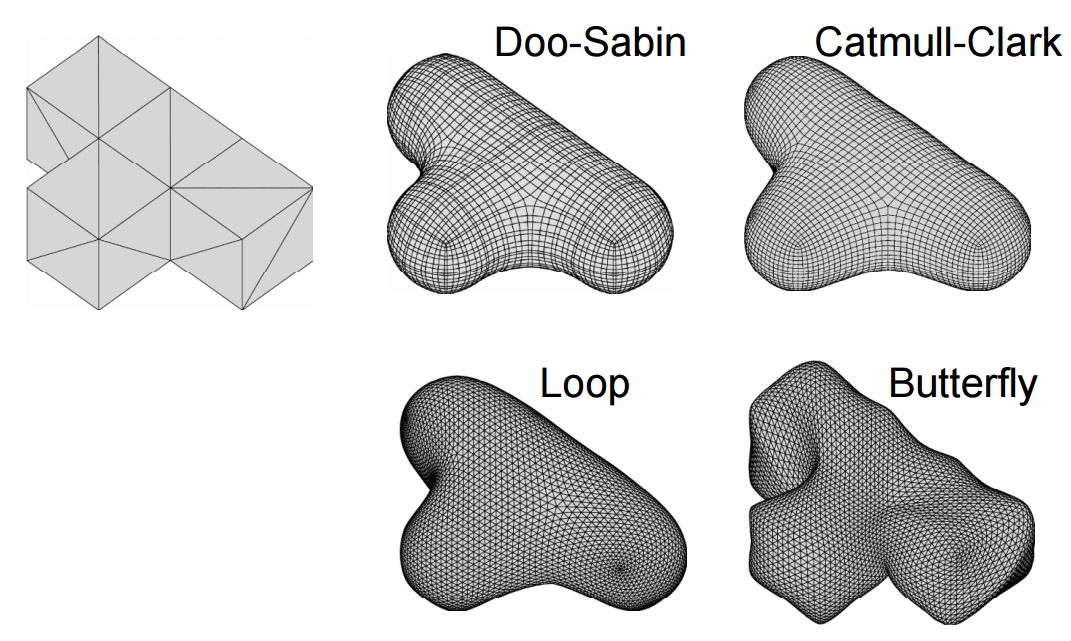
\includegraphics[width=0.9\textwidth]{content/media/sd_overview.png}
  \caption{Vergleich der Unterteilungsalgorithmen \cite{Standford.24.07.2015}}
  \label{fig:sd_comp}
\end{figure}

\section{Auswahl der Unterteilungsalgorithmen}

Für das Projekt sollen folgende Algorithmen implementiert werden:
\begin{itemize}
	\item Catmull-Clark
	\item Loop
	\item Doo-Sabin
	\item Butterfly
\end{itemize}


